% Wczytanie szablonu
\documentclass[nostrict]{Szablon}

% Definicja dokumentu
\usepackage[unicode=true]{hyperref}
\newcommand\PDFtitle{	
To jest szablon (mam nadzieję)}
\newcommand\PDFauthors{Jan Kąwałski}
\hypersetup{
  pdftitle={\PDFtitle},
  pdfauthor={\PDFauthors},
}

% \usepackage{textcomp}
\usepackage{array}
% pakiet stosowany do url'i w bibliografii, zamienia odnośniki na ładnie sformatowane
\usepackage{url}
% pakiety służące do numerowania i tworzenia algorytmów
\usepackage{algorithmic}
\usepackage{algorithm}
% redefinicja etykiety nagłówkowej listy algorytmów, domyślna jest po angielsku
\renewcommand{\listalgorithmname}{Spis algorytmów}

% pakiet do wyliczania skali, przydatny przy dużych obrazkach
\usepackage{pgf}
% tworzenie listingów
\usepackage{listings}
% tworzenie figur wewnątrz figur
\usepackage{subfig}

% makro umożliwiające otaczanie symboli okręgami
\usepackage{tikz}
% brak justowania tekstu (bazą okręgu będzie linia tekstu)
\newcommand*\mycirc[1]{%
  \begin{tikzpicture}
    \node[draw,circle,inner sep=1pt] {#1};
  \end{tikzpicture}}

% pionowe justowanie tekstu, środek okręgu pokrywa się ze środkiem tekstu
\newcommand*\mycircalign[1]{%
  \begin{tikzpicture}[baseline=(C.base)]
    \node[draw,circle,inner sep=1pt](C) {#1};
  \end{tikzpicture}}

% zmiana nazwy twierdzeń i lematów
\newtheorem{theorem}{Twierdzenie}[section]
\newtheorem{lemma}[theorem]{Lemat}

% redefinicja dowodu - pogrubiony
\renewenvironment{proof}[1][Dowód]{\begin{trivlist}
\item[\hskip \labelsep {\bfseries #1}]}{\end{trivlist}}
% \newenvironment{definition}[1][Definicja]{\begin{trivlist}
% \item[\hskip \labelsep {\bfseries #1}]}{\end{trivlist}}
% \newenvironment{example}[1][Przykład]{\begin{trivlist}
% \item[\hskip \labelsep {\bfseries #1}]}{\end{trivlist}}
% \newenvironment{remark}[1][Uwaga]{\begin{trivlist}
% \item[\hskip \labelsep {\bfseries #1}]}{\end{trivlist}}

% redefinicja czarnego prostokąta zwyczajowo dodawanego na koniec dowodu - oryginał jest biały
\renewcommand{\qed}{\nobreak \ifvmode \relax \else
      \ifdim\lastskip<1.5em \hskip-\lastskip
      \hskip1.5em plus0em minus0.5em \fi \nobreak
      \vrule height0.75em width0.5em depth0.25em\fi}

% poniższymi instrukcjami można sterować co ma być numerowane a co nie i co ma być wyświetlane w spisie treści
% \setcounter{secnumdepth}{3}
% \setcounter{tocdepth}{5}

% definicja czcionki mniejszej niż tiny (domyślnie takiej małej nie ma)
% \usepackage{lmodern}
\makeatletter
  \newcommand\tinyv{\@setfontsize\tinyv{4pt}{6}}
\makeatother

% definicja jeszcze mniejszej czcionki
% \usepackage{lmodern}
\makeatletter
  \newcommand\tinyvv{\@setfontsize\tinyvv{3.5pt}{6}}
\makeatother

% pakiet do obsługi wielostronicowych tabel
\usepackage{longtable}
\setlength{\LTcapwidth}{\textwidth}

% \usepackage[section] {placeins}

\usepackage{multirow}

\usepackage{slantsc}


% Zmiana czcionki dla symulacji maszynopisu (verbatim)
\makeatletter
\renewcommand{\verbatim@font}{\ttfamily\small}
\makeatother

% Część właściwa pracy
\begin{document}

\includepdf{chapters/oswiadczenia/tytulowa.pdf}
% 
\includepdf{chapters/oswiadczenia/oswiadczenie.pdf}
\hfill
\pagebreak

\chapter*{Streszczenie}
% \addcontentsline{toc}{chapter}{STRESZCZENIE}  
Streszczeie ąęśćźżiół
\newline
\newline
\textbf{Słowa kluczowe:} 
Słowo kluczowe 1, Słowo kluczowe 2, Słowo kluczowe 3
\newline
\textbf{Dziedzina nauki i techniki, zgodnie z wymogami OECD: }
\newline
Nauki o komputerach i informatyka


\chapter*{Abstract}
% \addcontentsline{toc}{chapter}{ABSTRACT}  
Abstract in english.
\newline
\newline
\textbf{Keywords:}
Keyword 1, Keyword 2, Keyword 3
\newline
\textbf{Field of science and technology in accordance with OECD requirements: } \newline
Computer Science and Information technology
\addcontentsline{toc}{chapter}{SPIS TREŚCI}
\tableofcontents

\chapter*{WYKAZ WAŻNIEJSZYCH OZNACZEŃ I SKRÓTÓW}
\addcontentsline{toc}{chapter}{WYKAZ WAŻNIEJSZYCH OZNACZEŃ I SKRÓTÓW}

\textbf{Skrót 1} - Opis 1.


\textbf{Skrót 2} - Opis 2.


\chapter{WSTĘP I CEL PRACY}
\label{chap:introduction}
Wstępu wstępu - tutaj należy pokrótce opisać o co chodzi w pracy i wyraźnie wskazać cel pracy!
% \begin{figure}[H]
%     \centering
%     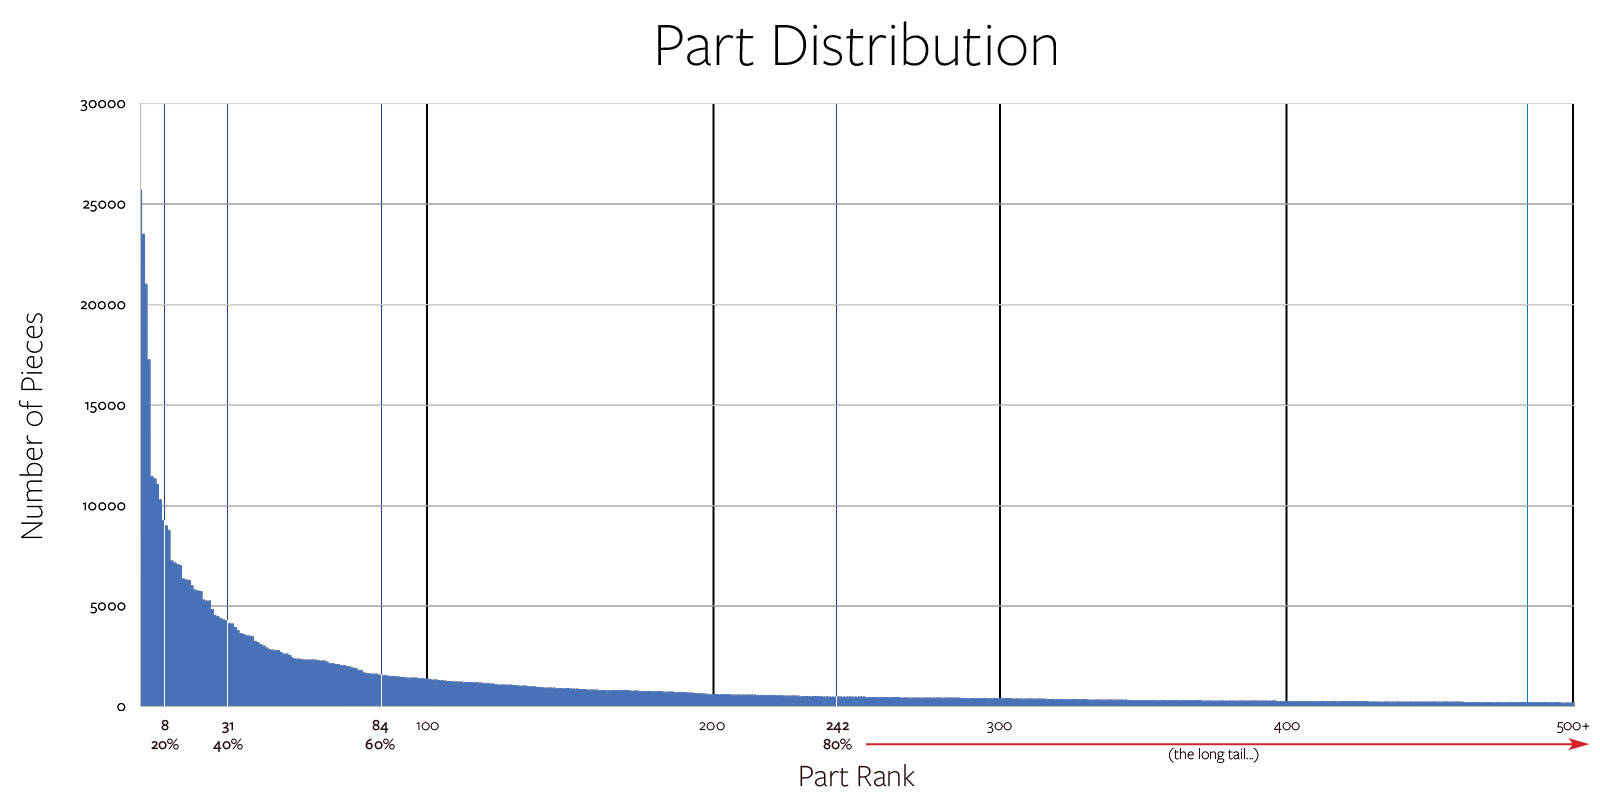
\includegraphics[width=1\textwidth]{images/part_dist.jpg}
%     \caption{Szacunkowa dystrybucja klas klocków kupionych w latach 2015-2020\cite{dist}}
%     \label{fig:part_dist}
% \end{figure}
% Na wykresie \ref{fig:part_dist} terefere.
\section{Cel pracy}
Mój super cel. 
\section{Układ pracy}
Układ pracy jest następujący...


\chapter{PODSTAWOWE ELEMENTY}

To jest rozdział.

\section{Podrozdziały}

W Latexu w klasie dokumentów \textbf{book} wyróżniamy rozdziały (\textbf{chapter}), podrozdziały \textbf{section}, podpodrozdziały \textbf{subsection}, podpodpodrozdziały \textbf{subsubsection} i paragrafy (\textbf{paragraph}). Podpodpodrozdziały i paragrafy domyślnie nie są numerowane ani nie występują w spisie treści. Zachowanie to można zmienić poprzez funkcję \textbf{setcounter} umieszczaną w preambule. Wykomentowany przykład można znaleźć w kodzie tego dokumentu.

Obecnie znajdujemy się na poziomie podrozdziału. Pozostałe przykłady poniżej.

\subsection{Podpodrozdział}

To jest podpodrozdział.

\subsubsection{Podpodpodrozdział}

To jest podpodpodrozdział. On nie jest domyślnie numerowany i nie występuje w spisie treści.

\paragraph{Paragraf}

A to jest paragraf. On również nie jest domyślnie numerowany i nie występuje w spisie treści.

\section{Podstawowe elementy typograficzne}

\subsection{Twarda spacja}

Twarda spacja jest bardzo istotnym elementem, gdyż zabrania Latex'owi łamanie linii w miejscu jej wystąpienia, a tym samym pozwoli na niejako ,,sklejenie'' wyrazów ze sobą. Dzięki temu możemy uniknąć tzw.\ sierot (pojedynczych znaków na końcu wiersza). W Latex twardą spację umieszcza się wstawiając znak tyldy~(\textasciitilde). Zapisujemy to więc np.\ tak: ,,dokument, w{\textasciitilde}którym''.

\subsection{Formatowanie tekstu}

Aby zapewnić poprawny wygląd tekstu należy pamiętać o kilku rzeczach:

\begin{itemize}
 \item Linia poprzedzona procentem to komentarz.
 \item Poprzedzaniu spacji występującej po kropce kończącej skrót znakiem ucieczki, odstęp będzie wtedy taki, jak odstęp między wyrazami a~nie między zdaniami. Przykładowo zapis ,,np. tekst'' vs. ,,np.\ tekst''. Ten drugi jest poprawny, a zapisany został tak: ,,np.$\backslash$~tekst''.
 \item Skróty pisane wielkimi literami kończące zdanie powinny posiadać {$\backslash$}@ przed kropką kończącą zdanie, np.\ OCS{$\backslash$}@\@. Spowoduje to potraktowanie spacji jako spacji międzyzdaniowej z nie międzywyrazowej.
 \item Cudzysłowie zawsze tworzymy używając podwójnego przecinka jako symbolu otwierającego cudzysłów, oraz podwójnego apostrofu zamykającego cudzysłów.
 \item Kursywę uzyskujemy za pomocą słowa kluczowego {$\backslash$}textit, co w efekcie daje \textit{tekst kursywą}. Pogrubiony \textbf{używamy słowa kluczowego textbf}. Każdorazowo tekst mający być napisany danym krojem otaczamy nawiasami klamrowymi.
 \item Myślnik (--) tworzymy poprzez umieszczenie bezpośrednio po sobie dwu kresek (minusy). Różnica między nimi jest zasadnicza. Pojedynczy myślnik generuje krótką kreskę (-), podwójny długą (--), potrójny najdłuższą (---).
 \item Odwołania do różnych elementów dokumentu robimy poprzez słowo kluczowe \textbf{ref()}. Jako jego parametr wstawiamy nazwę zdefiniowaną za pomocą słowa kluczowego \textbf{label()}. Należy pamiętać, że odwołanie zwraca jedynie numer elementu, słowo opisowe, jak np.\ rozdział czy rysunek należy dodać samodzielnie. Polecam tutaj przyjąć jakąś konwencję i się jej trzymać w całym dokumencie. Tak samo należy postępować w przypadku etykiet.
 \item Latex doskonale radzi sobie z dzieleniem wyrazów na końcach linii, jednak czasami zachodzi konieczność wymuszenia podziału w określonym miejscu. W tym celu należy zastosować konstrukcję $\backslash$-. Latex takiego ukośnika nie wydrukuje dopóty, dopóki rzeczywiście w tym miejscu nie zostanie wykonane przeniesienie części wyrazu. Możliwe jest dodanie wielu podziałów w jednym wyrazie. Użyte wtedy zostanie to, które spowoduje wygenerowania ,,najładniejszego'' tekstu.
\end{itemize}

\section{Podział linii i paragrafy}
\label{podzial}

Nowy paragraf rozpoczyna się poprzez wstawienie jednej wolnej linii. Latex automatycznie wygeneruje wcięcie. Należy pamiętać, że pierwszy paragraf, zgodnie ze standardami drukarskimi, nie ma wcięcia! Możemy tym sterować za pomocą poleceń \textbf{noindent} (brak wcięcia) oraz \textbf{indent} (dodatkowe wcięcie).

Jeżeli chcemy po prostu zrobić nową linię, bez tworzenia nowego paragrafu używamy konstrukcji $\backslash\backslash$. Efekt będzie taki, że paragraf\\
będzie kontynuowany w nowej linii. Nie spowoduje to jednak rozciągnięcia poprzedniej linii. Zostanie ona przerwana tam gdzie tego sobie zażyczymy i kontynuowana w nowej linijce.

A co w przypadku, gdy chcemy z jakiegoś powodu przerwać linię, ale wymusić justowanie tekstu? Weźmy dla przykładu fragment:

Trzecim istotnym aspektem jest stosowana w~trakcie wytwarzania ontologii metodologia pracy~\cite{boinski2012kaskbook,boinski2011security}. Zastosowanie jednej z~uznawanych metodologii, takich jak Methontology, NeOn czy metodologia opracowana przez Noy~i~McGuiness, znacząco wpływa na jakoś uzyskanego produktu. Wspomniane metodologie w~dużej mierze uwzględniają potrzebę przyszłej integracji wiedzy, a~w połączeniu z~narzędziami typu Protégé czy OCS~\cite{boinski2007kaskbook,boinski2009ocs,boinski2010zespolowa}, pozwalają na tworzenie spójnych i~formalnie oraz logicznie poprawnych ontologii.

Tekst zostaje bardzo brzydko złamany w środku odnośników do cytowań. Użycie podwójnego po słowie ,,metodologia'' w pierwszym zdaniu ukośnika da nam natomiast taki efekt:

Trzecim istotnym aspektem jest stosowana w~trakcie wytwarzania ontologii metodologia \\ pracy~\cite{boinski2012kaskbook,boinski2011security}. Zastosowanie jednej z~uznawanych metodologii, takich jak Methontology, NeOn czy metodologia opracowana przez Noy~i~McGuiness, znacząco wpływa na jakoś uzyskanego produktu. Wspomniane metodologie w~dużej mierze uwzględniają potrzebę przyszłej integracji wiedzy, a~w połączeniu z~narzędziami typu Protégé czy OCS~\cite{boinski2007kaskbook,boinski2009ocs,boinski2010zespolowa}, pozwalają na tworzenie spójnych i~formalnie oraz logicznie poprawnych ontologii.

Też nie ładnie, gdyż linijka jest niewyjustowana. Z pomocą przychodzi nam tutaj komenda \textbf{linebreak[]}, gdzie w nawiasie kwadratowym podajemy liczbę od 1 do 4 określająca jak bardzo zależy nam na tym, by linia została złamana w tym miejscu (4 to najwyższa wartość). Efekt jest następujący:

Trzecim istotnym aspektem jest stosowana w~trakcie wytwarzania ontologii metodologia \linebreak[4] pracy~\cite{boinski2012kaskbook,boinski2011security}. Zastosowanie jednej z~uznawanych metodologii, takich jak Methontology, NeOn czy metodologia opracowana przez Noy~i~McGuiness, znacząco wpływa na jakoś uzyskanego produktu. Wspomniane metodologie w~dużej mierze uwzględniają potrzebę przyszłej integracji wiedzy, a~w połączeniu z~narzędziami typu Protégé czy OCS~\cite{boinski2007kaskbook,boinski2009ocs,boinski2010zespolowa}, pozwalają na tworzenie spójnych i~formalnie oraz logicznie poprawnych ontologii.

Jeżeli z jakiegoś powodu potrzebujemy nową linię to używamy komendy \textbf{newpage}. \newpage Tekst występujący po niej znajdzie się na nowej stronie. Rozdziały itp.\ automatycznie generują nową stronę, przy czym w układzie dwustronnym nowy rozdział zawsze zacznie się od nieparzystej strony.

\section{Środowisko matematyczne}

Środowisko matematyczne otwieramy i zamykamy znakiem \$. Niektóre funkcje można używać tylko wewnątrz takiego środowiska. Przykładem niech będzie funkcja \textbf{mathcal} zamieniająca duże litery w symbole o charakterystycznym kroju, stosowanym do opisywania stałych, np.\ $\mathcal{O}$ czy $\mathcal{R(D,P,T,S,U,I)}$. Pamiętać należy, że zamienione zostaną wszystkie litery w wyrażeniu występującym wewnątrz nawiasów klamrowych.

Niektóre konstrukcje, np.\ równania, automatycznie włączają tryb matematyczny. Równania dobrze jest opisać, przykład przedstawia Równanie~\ref{eq:przyklad}.

\begin{equation}
  \mathcal{O(K,B,C,R)}
  \label{eq:przyklad}
\end{equation}

gdzie:\\
$\mathcal{K}$ - zbiór klas wchodzących w~skład ontologii,\\
$\mathcal{B}$ - zbiór bytów wchodzących w~skład ontologii,\\
$\mathcal{C}$ - zbiór komentarzy przypisanych do klas $\mathcal{K}$ i~bytów $\mathcal{B}$ wchodzących w~skład ontologii,\\
$\mathcal{R}$ - zbiór relacji wiążących elementy ontologii.


W równaniach możemy stosować różne dodatkowe symbole oraz np.\ wyrównywać je do określonego miejsca. Służy do tego blok typu \textbf{split}, a sam punkt wyrównania określony jest ampersandem (\&). Przykład zastosowania prezentuje równanie~\ref{eq:split_ex}.

\begin{equation}
  \label{eq:split_ex}
  \begin{split}
    \forall {x_1 \leq y_1, x_2 \leq y_2}&: f(x_1+x_2,y_1+y_2)\\ 
				  &= \frac{y_1}{y_1+y_2}f(x_1,y_1)+\frac{y_2}{y_1+y_2}f(x_2,y_2)
  \end{split}
\end{equation}

\subsection{Twierdzenia i dowody}

Linie 75 -- 93 nagłówka dokumentu definiują nowe nazwy sekcji twierdzeń i dowodów, oraz znacznik końca dowodu (taki czarny kwadracik). Dzięki nim można uzyskać ładnie wyglądające twierdzenia jak poniżej (Twierdzenie~\ref{eq:lin:theorem}). Zauważmy, że równanie dowodu nie jest równaniem numerowanym. Wszędzie tam, gdzie nie chcemy by rozdział czy dowolna inna sekcja była numerowana należy w jej nazwie użyć gwiazdki, np. \textbf{$\backslash$begin\{equation*\}}.

\begin{theorem}
 Podobieństwo pomiędzy pojęciami $A$ i~$B$ opisane jest stosunkiem ilości informacji niezbędnej do opisania ich wspólności znaczeniowej oraz ilością informacji niezbędnej do ich opisania (Równanie~\ref{eq:lin:theoremeq}).

 \begin{equation}
   sim_{lin}(A,B)=\frac{\log P(common(A,B))}{\log P(description(A,B))}
   \label{eq:lin:theoremeq}
 \end{equation}
 \label{eq:lin:theorem}
\end{theorem}

\begin{proof}
  \begin{equation*}
   \begin{split}
     f(x,y)&=f(x+0,y+(y-x))\\
	   &=\frac{x}{y}*f(x,x) +~\frac{y-z}{x}*f(0,y-z)\\
	   &=\frac{x}{y}*1 +~\frac{y-z}{x}*0\\
	   &=\frac{x}{y} \qed
   \end{split}
 \end{equation*}
\end{proof}

Inna ciekawa konstrukcja wykorzystująca tryb matematyczny do zapisania pewnego stwierdzenia:

Niech $A \subseteq T$, $C = N_y(A) \neq W$, a~$\alpha_y = \min_{a \in A, b\notin C} \{y(a) +~y(b) - q(a, b)\}$ oraz

\[ y'(v) = \left\{ \begin{array}{ll}
                y(v) - \alpha_y & \mbox{jeżeli $v \in A$} \\
                y(v) +~\alpha_y & \mbox{jeżeli $v \in C$} \\
                y(v)            & \mbox{w innych przypadkach}
               \end{array}
       \right. \]

Zapis ten, acz skomplikowany, pozwala na reprezentację złożonych reguł matematycznych w postaci ładnie ułożonych i wyrównanych wierszy. Reguły \textbf{left} oraz \textbf{right} pozwalają na utworzenie nawiasów klamrowych, których rozmiar będzie automatycznie dostosowywany do rozmiaru elementu, jakie mają zawierać.

\chapter{RYSUNKI, TABELE I INNE PODSTAWOWE KONSTRUKCJE}
\enlargethispage{20pt}
\section{Rysunki}
\label{rysunki}
Obrazki wstawiamy do dokumentu za pośrednictwem sekcji \textbf{figure}. Przykładowy wyśrodkowany rysunek z etykietą i opisem to Rys.~\ref{fig:obrazek}.

\begin{figure}[!h]
\centering

\includegraphics[width=0.7\textwidth]{images/obrazek.png}
\caption{Opis do obrazka.}
\label{fig:obrazek}
\end{figure}

W podanym przykładzie obrazek będzie wyśrodkowany, o szerokości odpowiadającej 70\% szerokości tekstu. Plik obrazka znajduje się w katalogu images i nazywa się obrazek.png. Latex dołoży starań, żeby umieścić go w tym miejscu (znacznik h w definicji figury). Wykrzyknik oznacza, że Latex bardzo się postara by obrazek tu był. Opisy obrazków zawsze znajdują się pod obrazkiem.

Latex potrafi wygenerować spis wszystkich numerowanych figur i umieścić go w miejscu, gdzie użyjemy polecenia \textbf{listoffigures}.

\subsection{Wielostronicowe obrazki}

Czasami zdarza się, że obrazek jest tak duży, że umieszczenie go na jednej stronie powoduje, że stanie się nieczytelny. Latex umożliwia pocięcie obrazka na kawałki, przeskalowanie i przetworzenie tych kawałków, oraz wyświetlenie ich w postaci następujących po sobie figur, gdzie tylko pierwsza wskazana będzie numerowana i uwzględniona w spisie rysunków. Przykład prezentuje Rys.~\ref{fig:duzy_obrazek}. Podpis pod każdą częścią będzie odmienny, numeracja będzie wspólna, w spisie wskazanie będzie do pierwszego z obrazków. Po szczegóły zapraszam do dokumentu w celu przeczytania komentarzy.


% definition of the scale of the picture
% here each part of the picture is rescaled
% so that it will fit page swidth
% 1255 is the original width of the picture
% later on we can use \ratio command as a macro
% that will rescale the fragment of the picture
\pgfmathsetmacro{\ratio}{\the\textwidth/1255}
% standard figure environment
\begin{figure}[h]
% centered
 \centering
% scaled by ratio fragment of the picture
% includegraphic*[vieport=lower_left_x lower_left_y upper_right_x upper_right_y]{image}
% in here we print upper part of the picture
   \scalebox{\ratio}{\includegraphics*[viewport=0 1951 1255 3795]{images/duzy_obrazek.png}}
% and the caption
   \caption{Bardzo duży obrazek}
\end{figure}

\begin{figure}[h]
% this tells Latex that this float is continuation of the previous one
% this way new number will not be assigned
\ContinuedFloat
% here we print lower part of the picture
 \centering
   \scalebox{\ratio}{\includegraphics*[viewport=0 0 1255 1951]{images/duzy_obrazek.png}}
 \caption[]{(ciąg dalszy)}
 \label{fig:duzy_obrazek}
\end{figure}

Analogicznie można również wstawiać i dzielić na kawałki obrazki zawarte w plikach pdf. Tutaj warto jednak rozmiary w mm podać, gdyż rozmiar po pikselach potrafi się rozjechać. Przykład efektu działania znajduje się na obrazku~\ref{fig:mw}. Przykład pochodzi od mgr inż.\ Michała Wójcika.

\begin{figure}[htb!]
  \centering
  \includegraphics*[viewport=0 153mm 175mm 306mm, scale=0.85]{images/producer-supervisor-perofmers.pdf}
  \caption{Duży obrazek w pdf}
\end{figure}

\begin{figure}[htb!]
  \ContinuedFloat
  \centering
  \includegraphics*[viewport=0 0 175mm 153mm, scale=0.85]{images/producer-supervisor-perofmers.pdf}
  \caption{(continued - UWAGA - brak [] po caption powoduje widoczność podpisu kontynuacji na wykazie!)}
  \label{fig:mw}
\end{figure}

Należy zauważyć, że Latex dołoży wszelkich starań, by obrazek umieścić tam gdzie go sobie zażyczyliśmy. Czasami jest to jednak niemożliwe, ze względu na zbyt małą ilość tekstu i niestety trzeba pokombinować. Typowe zabiegi to próba dodania znacznika [!h] przy definicji figury, wstawienie obrazka wcześniej w tekście czy też lekka zmiana jego rozmiaru.

\subsection{Wymuszanie renderowania obrazków do pewnego miejsca}

Czasami zdarza się, że Latex zbyt długo zwleka z renderowanie obrazków, przez co w pamięci podręcznej zaczyna brakować miejsca. Najczęściej problem ten występuje, gdy dokument zawiera bardzo dużo obrazków, a raczej niewiele tekstu, lub relacje pomiędzy rozmiarami obrazków a liczbą słów są zachwiane i nie jest możliwe ich poprawne rozlokowanie.

Wszystkie zaległe obrazki zawsze renderowane są na koniec rozdziału, jednak ich duże nagromadzenie może spowodować błąd przepełnienia pamięci. Czasami też koniec rozdziału jest zbyt odległym miejscem i lepiej po prostu wymusić renderowanie zaległych ramek w określonym miejscu. Służy temu komenda \textbf{$\backslash$clearpage}. Jej zastosowanie spowoduje renderowanie wszystkich, do tej pory nierozlokowanych obrazków.

\section{Listingi}
\label{listingi}
\enlargethispage{-5cm}
Tworzenie listingów umożliwia pakiet \textbf{listings}. Należy zwrócić uwagę, że etykiety i opisy listingów dodaje się w dośc specyficzny sposób jako parametry do bloku \textbf{lstlisting} (patrz kod dokumentu). Używając funkcji \textbf{lstset} możliwa jest zmiana kroju czcionki na inną niż reszty dokumentu. W przykładzie (Listing~\ref{kod:listingA}) zmniejszono czcionkę do rozmiaru indeksu dolnego.

\lstset{basicstyle=\scriptsize}
\begin{lstlisting}[frame=single,caption={Przykładowy listing},label=kod:listingA]
<?xml version="1.0"?>

<!DOCTYPE rdf:RDF [
 <!ENTITY owl "http://www.w3.org/2002/07/owl#" >
 <!ENTITY xsd "http://www.w3.org/2001/XMLSchema#" >
 <!ENTITY rdfs "http://www.w3.org/2000/01/rdf-schema#" >
 <!ENTITY rdf "http://www.w3.org/1999/02/22-rdf-syntax-ns#" >
]>

<rdf:RDF xmlns="http://kask.eti.pg.gda.pl/securityA.owl#"
 xml:base="http://kask.eti.pg.gda.pl/securityA.owl"
 xmlns:rdfs="http://www.w3.org/2000/01/rdf-schema#"
 xmlns:owl="http://www.w3.org/2002/07/owl#"
 xmlns:xsd="http://www.w3.org/2001/XMLSchema#"
 xmlns:rdf="http://www.w3.org/1999/02/22-rdf-syntax-ns#">
 <owl:Ontology rdf:about="http://kask.eti.pg.gda.pl/securityA.owl"/>

 <!-- 
 ///////////////////////////////////////////////////////////////////////////////////////
 //
 // Classes
 //
 ///////////////////////////////////////////////////////////////////////////////////////
 -->

 <!-- http://kask.eti.pg.gda.pl/securityA.owl#DSA -->

 <owl:Class rdf:about="http://kask.eti.pg.gda.pl/securityA.owl#DSA">
  <rdfs:subClassOf rdf:resource="http://kask.eti.pg.gda.pl/securityA.owl#asymetryczne"/>
 </owl:Class>

  
 <!-- http://kask.eti.pg.gda.pl/securityA.owl#RSA -->

 <owl:Class rdf:about="http://kask.eti.pg.gda.pl/securityA.owl#RSA">
  <rdfs:subClassOf rdf:resource="http://kask.eti.pg.gda.pl/securityA.owl#asymetryczne"/>
 </owl:Class>

  
 <!-- http://kask.eti.pg.gda.pl/securityA.owl#asymetryczne -->

 <owl:Class rdf:about="http://kask.eti.pg.gda.pl/securityA.owl#asymetryczne"/>
  

 <!-- http://kask.eti.pg.gda.pl/securityA.owl#symetryczne -->

 <owl:Class rdf:about="http://kask.eti.pg.gda.pl/securityA.owl#symetryczne"/>
</rdf:RDF>

\end{lstlisting}

\section{Algorytmy}
\label{algorytmy}
Pakiety \textbf{algorithmic} oraz \textbf{algorithm} dostarczają środowiska do definiowania algorytmów. Można za ich pomocą definiować zarówno pseudokod jak i algorytmy ogólne. Pseudokod przedstawia Algorytm~\ref{tboi:alg}. Przykładową ogólną reprezentację algorytmu Levenshteina obrazuje Algorytm~\ref{tboi:alg_leven}.

\begin{algorithm}
 \floatname{algorithm}{Algorytm}
 \caption{Pseudokod prezentujący jakiś bezsensowny algorytm}
 \label{tboi:alg}
 \begin{algorithmic}[1]
\STATE \textbf{program} FancyProgram \{

\STATE \textbf{function} superFunkcja(List listA) \{

\FORALL{element :~listA.getElements()}
\STATE int result = storeElement(element);
\IF{result == SUCCESS}
\STATE double number = result*element;
\ELSIF{result == FAILURE}
\STATE double number = result/element;
\ENDIF
\ENDFOR
\STATE \}

\STATE input List elements;
\STATE output number;

\STATE superFunkcja(elements);
\RETURN number;
\STATE \}
 \end{algorithmic}
\end{algorithm}

\begin{algorithm}
 \floatname{algorithm}{Algorytm}
 \caption{Algorytm Levenshteina}
 \label{tboi:alg_leven}
%  \begin{algorithmic}[1]
\begin{enumerate}
 \item Niech $n = \textit{długość}(s)$ a~$m = \textit{długość}(t)$.
 \item Jeżeli $n == 0$ zwróć m~i zakończ działanie.
 \item Jeżeli $m == 0$ zwróć n~i zakończ działanie.
 \item Utwórz macierz $d$ o~$m+1$ wierszach indeksowanych od $0$ do $m$ oraz $n+1$ kolumnach indeksowanych od $0$ do $n$, pierwszy wiersz zainicjuj wartościami od $0$ do $n$ a~pierwszą kolumnę od $0$ do $m$.
 \item Porównaj każdy znak pierwszego ciągu, indeksowany za pomocą $i$, z~każdym znakiem drugiego ciągu, indeksowanym za pomocą $j$. Dla każdego porównania:
\begin{enumerate}
 \item jeżeli $s[i]$ jest identyczne z~$t[j]$, $koszt = 0$, w~przeciwnym wypadku $koszt = 1$,
 \item ustaw wartość komórki $d[i,j]$ macierzy na wartość minimalną spośród:
\begin{itemize}
 \item $d[i-1,j] +~1$,
 \item $d[i,j-1] +~1$,
 \item $d[i-1,j-1] +~koszt$.
\end{itemize}
\end{enumerate}
 \item Odczytaj odległość $dist_{lev}(s,t)$ z~komórki $d[n,m]$.
\end{enumerate}
%\end{algorithmic}
\end{algorithm}

Podobnie jak w przypadku rysunków, algorytmy są automatycznie rozlokowywane w tekście przez system Latex.

\section{Tabele}

Latex pozwala na konstruowanie bardzo rozbudowanych tabel. Pełny opis możliwości znaleźć można w sieci Internet, a samo zagadnienie jest bardzo skomplikowane. Prosty przykład prezentuje Tabela~\ref{tab:tab1}.

\begin{table}[h]
\caption{Opis tabelki}
\label{tab:tab1}
 \centering
\begin{tabular}{|c|p{4.5cm}|p{6cm}|}
  \hline
  Pole 1 & Pole 2 & Pole 3\\
  \hline
  1 & Pojęcie & Opis tegoż pojęcia\\
  \hline
  2 & Pojęcie & Opis tegoż pojęcia\\
  \hline
\end{tabular}
% \vspace{-0.5cm}
\end{table}

Pakiet \textbf{longtable} pozwala na generowanie ogromnych tabel rozłożonych na kilka stron.

% this changes spacing between table rows, default is one, needs to be reset after the table!
\renewcommand{\arraystretch}{0.85}
% longtable definition, headers are defined in the same manner as normal table
% here we change fontsize in each collumn to size smaller than tine defined in the preamble
% all keywords within the table definition are the same as in standard table
\begin{longtable}[h!]{|>{\tinyv}l|>{\tinyv}c|>{\tinyv}c|>{\tinyv}c|>{\tinyv}c|>{\tinyv}c|>{\tinyv}c|>{\tinyv}c|>{\tinyv}c|>{\tinyv}c|>{\tinyv}c|}
\caption{Bardzo długa tabela (główna etykieta)\label{tab:long_table}}\\
\endfirsthead
\caption[]{(ciąg dalszy -- ten tekst pokazywać się będzie na kolejnych stronach)}\\
\endhead
\hline
Lemma B~& \multicolumn{5}{>{\tinyv}c|}{Agency} & \multicolumn{5}{>{\tinyv}c|}{Area} \\
\hline
Lemma A~& $max(P_{lex},P_{sem})$ & $P_{kom}$ & $P_{str}$ & $P_{sk}$ & Wynik & $max(P_{lex},P_{sem})$ & $P_{kom}$ & $P_{str}$ & $P_{sk}$ & Wynik \\
\hline
Asset & 0,30 & 0,00 & 0,06 & 0,02 & Różne & 0,40 & 0,00 & 0,06 & 0,02 & Różne \\
\hline
Attack & 0,33 & 0,00 & 0,09 & 0,03 & Różne & 0,33 & 0,00 & 0,09 & 0,03 & Różne \\
\hline
Circumstance & 0,37 & 0,00 & 0,00 & 0,00 & Różne & 0,85 & X~& X~& X~& Rodzeństwo \\
\hline
Continuity & 0,31 & 0,00 & 0,13 & 0,04 & Różne & 0,42 & 0,00 & 0,13 & 0,04 & Różne \\
\hline
Error & 0,32 & 0,00 & 0,08 & 0,03 & Różne & 0,35 & 0,00 & 0,08 & 0,03 & Różne \\
\hline
Event & 0,46 & 0,00 & 0,10 & 0,03 & Różne & 0,40 & 0,00 & 0,10 & 0,03 & Różne \\
\hline
Group & 0,60 & 0,00 & 0,00 & 0,00 & Różne & 0,55 & 0,00 & 0,00 & 0,00 & Różne \\
\hline
Harm & 0,37 & 0,00 & 0,00 & 0,00 & Różne & 0,42 & 0,00 & 0,00 & 0,00 & Różne \\
\hline
Mission & 0,46 & 0,00 & 0,10 & 0,03 & Różne & 0,19 & 0,00 & 0,10 & 0,03 & Różne \\
\hline
Operation & 0,83 & X~& X~& X~& Rodzeństwo & 0,43 & 0,00 & 0,50 & 0,15 & Różne \\
\hline
Organization & 0,72 & X~& X~& X~& B~podrzędne A~& 0,35 & 0,00 & 0,10 & 0,03 & Różne \\
\hline
Potential & 0,36 & 0,00 & 0,00 & 0,00 & Różne & 0,41 & 0,00 & 0,00 & 0,00 & Różne \\
\hline
Risk & 0,32 & 0,00 & 0,17 & 0,05 & Różne & 0,20 & 0,00 & 0,17 & 0,05 & Różne \\
\hline
Security & 0,65 & 0,00 & 0,00 & 0,00 & Różne & 0,40 & 0,00 & 0,00 & 0,00 & Różne \\
\hline
Threat & 0,28 & 0,00 & 0,00 & 0,00 & Różne & 0,50 & 0,00 & 0,00 & 0,00 & Różne \\
\hline
Value & 0,30 & 0,00 & 0,11 & 0,03 & Różne & 0,47 & 0,00 & 0,11 & 0,03 & Różne \\
\hline
Vulnerability & 0,31 & 0,00 & 0,00 & 0,00 & Różne & 0,42 & 0,00 & 0,00 & 0,00 & Różne \\
\hline
Weakness & 0,34 & 0,00 & 0,11 & 0,03 & Różne & 0,44 & 0,00 & 0,11 & 0,03 & Różne \\
\hline \hline
Lemma B~& \multicolumn{5}{>{\tinyv}c|}{Asset} & \multicolumn{5}{>{\tinyv}c|}{Attack} \\
\hline
Lemma A~& $max(P_{lex},P_{sem})$ & $P_{kom}$ & $P_{str}$ & $P_{sk}$ & Wynik & $max(P_{lex},P_{sem})$ & $P_{kom}$ & $P_{str}$ & $P_{sk}$ & Wynik \\
\hline
Asset & 1,00 & X~& X~& X~& Tożsame & 0,17 & 0,00 & 0,39 & 0,12 & Różne \\
\hline
Attack & 0,17 & 0,00 & 0,85 & 0,25 & Różne & 1,00 & X~& X~& X~& Tożsame \\
\hline
Circumstance & 0,32 & 0,34 & 0,00 & 0,24 & Różne & 0,25 & 0,00 & 0,00 & 0,00 & Różne \\
\hline
Continuity & 0,27 & 0,00 & 0,50 & 0,15 & Różne & 0,26 & 0,00 & 0,25 & 0,08 & Różne \\
\hline
Error & 0,48 & 0,25 & 0,47 & 0,31 & Różne & 0,45 & 0,00 & 0,27 & 0,08 & Różne \\
\hline
Event & 0,32 & 0,20 & 0,64 & 0,33 & Różne & 0,51 & 0,00 & 0,42 & 0,13 & Różne \\
\hline
Group & 0,13 & 0,00 & 0,00 & 0,00 & Różne & 0,31 & 0,00 & 0,00 & 0,00 & Różne \\
\hline
Harm & 0,33 & 0,26 & 0,00 & 0,18 & Różne & 0,51 & 0,00 & 0,00 & 0,00 & Różne \\
\hline
Mission & 0,29 & 0,00 & 0,44 & 0,13 & Różne & 0,77 & X~& X~& X~& Rodzeństwo \\
\hline
Operation & 0,31 & 0,00 & 0,15 & 0,05 & Różne & 0,95 & X~& X~& X~& B~podrzędne A~\\
\hline
Organization & 0,55 & 0,31 & 0,35 & 0,33 & Różne & 0,76 & X~& X~& X~& Rodzeństwo \\
\hline
Potential & 0,32 & 0,22 & 0,00 & 0,16 & Różne & 0,46 & 0,00 & 0,00 & 0,00 & Różne \\
\hline
Risk & 0,20 & 0,29 & 0,46 & 0,34 & Różne & 0,40 & 0,00 & 0,18 & 0,05 & Różne \\
\hline
Security & 0,31 & 0,00 & 0,00 & 0,00 & Różne & 0,39 & 0,00 & 0,00 & 0,00 & Różne \\
\hline
Threat & 0,33 & 0,23 & 0,00 & 0,16 & Różne & 0,40 & 0,00 & 0,00 & 0,00 & Różne \\
\hline
Value & 0,64 & 0,00 & 0,38 & 0,11 & Różne & 0,20 & 0,00 & 0,14 & 0,04 & Różne \\
\hline
Vulnerability & 0,27 & 0,31 & 0,00 & 0,22 & Różne & 0,08 & 0,00 & 0,00 & 0,00 & Różne \\
\hline
Weakness & 0,47 & 0,22 & 0,38 & 0,27 & Różne & 0,13 & 0,00 & 0,14 & 0,04 & Różne \\
\hline \hline
Lemma B~& \multicolumn{5}{>{\tinyv}c|}{Circumstance} & \multicolumn{5}{>{\tinyv}c|}{Countermeasure} \\
\hline
Lemma A~& $max(P_{lex},P_{sem})$ & $P_{kom}$ & $P_{str}$ & $P_{sk}$ & Wynik & $max(P_{lex},P_{sem})$ & $P_{kom}$ & $P_{str}$ & $P_{sk}$ & Wynik \\
\hline
Asset & 0,32 & 0,00 & 0,11 & 0,03 & Różne & 0,14 & 0,00 & 0,00 & 0,00 & Różne \\
\hline
Attack & 0,25 & 0,00 & 0,18 & 0,05 & Różne & 0,31 & 0,00 & 0,00 & 0,00 & Różne \\
\hline
Circumstance & 1,00 & X~& X~& X~& Tożsame & 0,21 & 0,00 & 0,00 & 0,00 & Różne \\
\hline
Continuity & 0,33 & 0,00 & 0,25 & 0,08 & Różne & 0,29 & 0,00 & 0,00 & 0,00 & Różne \\
\hline
Error & 0,27 & 0,00 & 0,17 & 0,05 & Różne & 0,21 & 0,00 & 0,00 & 0,00 & Różne \\
\hline
Event & 0,99 & X~& X~& X~& A~podrzędne B~& 0,26 & 0,00 & 0,00 & 0,00 & Różne \\
\hline
Group & 0,17 & 0,00 & 0,00 & 0,00 & Różne & 0,14 & 0,00 & 0,00 & 0,00 & Różne \\
\hline
Harm & 0,52 & 0,00 & 0,00 & 0,00 & Różne & 0,33 & 0,00 & 0,00 & 0,00 & Różne \\
\hline
Mission & 0,25 & 0,00 & 0,20 & 0,06 & Różne & 0,20 & 0,00 & 0,00 & 0,00 & Różne \\
\hline
Operation & 0,41 & 0,00 & 0,33 & 0,10 & Różne & 0,29 & 0,00 & 0,00 & 0,00 & Różne \\
\hline
Organization & 0,34 & 0,00 & 0,20 & 0,06 & Różne & 0,34 & 0,00 & 0,00 & 0,00 & Różne \\
\hline
Potential & 0,39 & 0,00 & 0,00 & 0,00 & Różne & 0,29 & 0,00 & 0,00 & 0,00 & Różne \\
\hline
Risk & 0,23 & 0,00 & 0,33 & 0,10 & Różne & 0,21 & 0,00 & 0,00 & 0,00 & Różne \\
\hline
Security & 0,49 & 0,00 & 0,00 & 0,00 & Różne & 0,73 & X~& X~& X~& Rodzeństwo \\
\hline
Threat & 0,21 & 0,00 & 0,00 & 0,00 & Różne & 0,29 & 0,00 & 0,00 & 0,00 & Różne \\
\hline
Value & 0,33 & 0,00 & 0,22 & 0,07 & Różne & 0,21 & 0,00 & 0,00 & 0,00 & Różne \\
\hline
Vulnerability & 0,43 & 0,00 & 0,00 & 0,00 & Różne & 0,21 & 0,00 & 0,00 & 0,00 & Różne \\
\hline
Weakness & 0,36 & 0,00 & 0,22 & 0,07 & Różne & 0,14 & 0,00 & 0,00 & 0,00 & Różne \\
\hline \hline
Lemma B~& \multicolumn{5}{>{\tinyv}c|}{Device} & \multicolumn{5}{>{\tinyv}c|}{Event} \\
\hline
Lemma A~& $max(P_{lex},P_{sem})$ & $P_{kom}$ & $P_{str}$ & $P_{sk}$ & Wynik & $max(P_{lex},P_{sem})$ & $P_{kom}$ & $P_{str}$ & $P_{sk}$ & Wynik \\
\hline
Asset & 0,08 & 0,00 & 0,00 & 0,00 & Różne & 0,32 & 0,13 & 0,39 & 0,21 & Różne \\
\hline
Attack & 0,37 & 0,00 & 0,00 & 0,00 & Różne & 0,51 & 0,00 & 0,64 & 0,19 & Różne \\
\hline
Circumstance & 0,21 & 0,00 & 0,00 & 0,00 & Różne & 0,99 & X~& X~& X~& B~podrzędne A~\\
\hline
Continuity & 0,27 & 0,00 & 0,00 & 0,00 & Różne & 0,32 & 0,00 & 0,25 & 0,08 & Różne \\
\hline
Error & 0,30 & 0,00 & 0,00 & 0,00 & Różne & 0,42 & 0,17 & 0,27 & 0,20 & Różne \\
\hline
Event & 0,34 & 0,00 & 0,00 & 0,00 & Różne & 1,00 & X~& X~& X~& Tożsame \\
\hline
Group & 0,13 & 0,00 & 0,00 & 0,00 & Różne & 0,24 & 0,00 & 0,00 & 0,00 & Różne \\
\hline
Harm & 0,40 & 0,00 & 0,00 & 0,00 & Różne & 0,51 & 0,18 & 0,00 & 0,12 & Różne \\
\hline
Mission & 0,24 & 0,00 & 0,00 & 0,00 & Różne & 0,37 & 0,00 & 0,21 & 0,06 & Różne \\
\hline
Operation & 0,27 & 0,00 & 0,00 & 0,00 & Różne & 0,57 & 0,00 & 0,29 & 0,09 & Różne \\
\hline
Organization & 0,41 & 0,00 & 0,00 & 0,00 & Różne & 0,41 & 0,22 & 0,13 & 0,20 & Różne \\
\hline
Potential & 0,22 & 0,00 & 0,00 & 0,00 & Różne & 0,67 & 0,14 & 0,00 & 0,10 & Różne \\
\hline
Risk & 0,26 & 0,00 & 0,00 & 0,00 & Różne & 0,41 & 0,18 & 0,18 & 0,18 & Różne \\
\hline
Security & 0,83 & X~& X~& X~& Rodzeństwo & 0,48 & 0,00 & 0,00 & 0,00 & Różne \\
\hline
Threat & 0,30 & 0,00 & 0,00 & 0,00 & Różne & 0,35 & 0,19 & 0,00 & 0,13 & Różne \\
\hline
Value & 0,18 & 0,00 & 0,00 & 0,00 & Różne & 0,32 & 0,00 & 0,14 & 0,04 & Różne \\
\hline
Vulnerability & 0,15 & 0,00 & 0,00 & 0,00 & Różne & 0,42 & 0,18 & 0,00 & 0,12 & Różne \\
\hline
Weakness & 0,25 & 0,00 & 0,00 & 0,00 & Różne & 0,35 & 0,23 & 0,14 & 0,21 & Różne \\
\hline \hline
Lemma B~& \multicolumn{5}{>{\tinyv}c|}{Group} & \multicolumn{5}{>{\tinyv}c|}{Harm} \\
\hline
Lemma A~& $max(P_{lex},P_{sem})$ & $P_{kom}$ & $P_{str}$ & $P_{sk}$ & Wynik & $max(P_{lex},P_{sem})$ & $P_{kom}$ & $P_{str}$ & $P_{sk}$ & Wynik \\
\hline
Asset & 0,13 & 0,00 & 0,00 & 0,00 & Różne & 0,33 & 0,00 & 0,00 & 0,00 & Różne \\
\hline
Attack & 0,31 & 0,00 & 0,00 & 0,00 & Różne & 0,51 & 0,00 & 0,00 & 0,00 & Różne \\
\hline
Circumstance & 0,17 & 0,00 & 0,00 & 0,00 & Różne & 0,52 & 0,00 & 0,00 & 0,00 & Różne \\
\hline
Continuity & 0,10 & 0,00 & 0,00 & 0,00 & Różne & 0,33 & 0,00 & 0,00 & 0,00 & Różne \\
\hline
Error & 0,20 & 0,00 & 0,00 & 0,00 & Różne & 0,45 & 0,00 & 0,00 & 0,00 & Różne \\
\hline
Event & 0,24 & 0,00 & 0,00 & 0,00 & Różne & 0,51 & 0,00 & 0,00 & 0,00 & Różne \\
\hline
Group & 1,00 & X~& X~& X~& Tożsame & 0,11 & 0,00 & 0,00 & 0,00 & Różne \\
\hline
Harm & 0,11 & 0,00 & 0,00 & 0,00 & Różne & 1,00 & X~& X~& X~& Tożsame \\
\hline
Mission & 0,46 & 0,00 & 0,00 & 0,00 & Różne & 0,26 & 0,00 & 0,00 & 0,00 & Różne \\
\hline
Operation & 0,17 & 0,00 & 0,00 & 0,00 & Różne & 0,39 & 0,00 & 0,00 & 0,00 & Różne \\
\hline
Organization & 0,87 & X~& X~& X~& A~podrzędne B~& 0,48 & 0,00 & 0,00 & 0,00 & Różne \\
\hline
Potential & 0,11 & 0,00 & 0,00 & 0,00 & Różne & 0,40 & 0,00 & 0,00 & 0,00 & Różne \\
\hline
Risk & 0,32 & 0,00 & 0,00 & 0,00 & Różne & 0,28 & 0,00 & 0,00 & 0,00 & Różne \\
\hline
Security & 0,43 & 0,00 & 0,00 & 0,00 & Różne & 0,50 & 0,00 & 0,00 & 0,00 & Różne \\
\hline
Threat & 0,17 & 0,00 & 0,00 & 0,00 & Różne & 0,25 & 0,00 & 0,00 & 0,00 & Różne \\
\hline
Value & 0,46 & 0,00 & 0,00 & 0,00 & Różne & 0,33 & 0,00 & 0,00 & 0,00 & Różne \\
\hline
Vulnerability & 0,09 & 0,00 & 0,00 & 0,00 & Różne & 0,44 & 0,00 & 0,00 & 0,00 & Różne \\
\hline
Weakness & 0,10 & 0,00 & 0,00 & 0,00 & Różne & 0,36 & 0,00 & 0,00 & 0,00 & Różne \\
\hline
\end{longtable}
% remember to reset table spacing!!!
\renewcommand{\arraystretch}{1}

\chapter{INNE PRZYDATNE KONSTRUKCJE}
\section{Symbole otoczone kółkiem}

Latex pozwala na tworzenie własnych znaków i symboli. W mojej rozprawie doktorskiej potrzebowałem zestawu symboli zamkniętych w okrąg, np.\ \mycircalign{+}, \mycircalign{-}, \mycircalign{k}. Za pomocą pakietu \textbf{tikz} zdefiniowałem dwa makra: \textbf{mycircalign} oraz \textbf{mycirc}. Pierwsze z nich otacza symbol kółkiem i wyrównuje powstały obrazek tak, by jego środek pokrywał się ze środkiem sąsiadujących znaków. Drugi układa elementy na linii tekstu, tak że spody znaków sąsiadujących i powstałego obrazka są wyrównane. Jak każde makro, również i te można używać zarówno w tekście jak i w środowisku matematycznym, tabelkach itp. (Równanie~\ref{eq:makro}).

\begin{equation}
  \mathcal{O}_3 = \mathcal{O}_1 \mycircalign{+} \mathcal{O}_2
  \label{eq:makro}
\end{equation}

\section{Tymczasowa zmiana rozmiaru strony}

Czasami zachodzi konieczność chwilowej zmiany rozmiaru strony, by np.\ udało się zmieścić jedną dodatkową linijkę tekstu. Możemy to wykonać za pomocą polecenia \textbf{enlargethispage\{\}}, gdzie jako parametr podajemy rozmiar oraz jednostkę. Należy pamiętać, że polecenie to musi zostać wydane odpowiednio wcześniej, by Latex zdążył zastosować nowy rozmiar strony. Najlepiej by te polecenie było bezpośrednio przed nową stroną, jednak zazwyczaj jest to kwestia poeksperymentowania. Wartość przekazana jako parametr może być także ujemna. Przykładowo strona zawierająca rozdział~\ref{listingi} została w niniejszym dokumencie pomniejszona o 5 cm wymuszając przeniesienie początku rozdziału~\ref{algorytmy} na następną stronę.

Strona zawierająca rozdział~\ref{rysunki} powiększono o~20~punktów, co pozwoliło uniknąć samotnej, pojedynczej linii tekstu kończącego akapit (tzw.\ wdowy) na następnej stronie. Takie drobne modyfikacje rozmiaru strony zazwyczaj są niezauważalne dla czytelnika a poprawiają ogólny układ dokumentu.

\section{Wpisy bibliograficzne}

Wpisy bibliograficzne przechowujemy w odrębnym pliku z rozszerzeniem\ .bib. Przykładowy plik został dołączony do tego dokumentu. Do pliku takiego należy dodawać odpowiedni sformatowane wpisy. Latex automatycznie posortuje je po nazwiskach autorów oraz do finalnego dokumentu dołączy tylko te wpisy,które posiadają odwołania w tekście! Można więc stworzyć kompletną bazę publikacji, a Latex użyje tylko to co potrzeba. Dodatkowo, dzięki użyciu pakietu \textbf{natbib} z parametrem \textbf{sort} (patrz preambuła dokumentu), numerki w odwołaniach również zostaną posortowane, niezależnie od kolejności podania odwołań. Przykład podano w rozdziale~\ref{podzial}.
\chapter{PODSUMOWANIE}
\label{chap:podsumowanie}
Podsumowanie pracy. 


% Bibliografia, ignorujemy overfull box, bo są długie URL
\hfuzz=50pt
\printbibliography[title=\bibliographyname]
\addcontentsline{toc}{chapter}{\bibliographyname}
\hfuzz=0pt

% Wykaz rysunków
\listoffigures
\addcontentsline{toc}{chapter}{\listfigurename}

% Wykaz tabel
\listoftables
\addcontentsline{toc}{chapter}{\listtablename}


\end{document}
